\documentclass[12pt, a4paper, simple]{eskdtext}

\usepackage{hyperref}
\usepackage{env}
\usepackage{_sty/gpi_lst}
\usepackage{_sty/gpi_toc}
\usepackage{_sty/gpi_t}
\usepackage{_sty/gpi_p}
\usepackage{_sty/gpi_u}

% Код
\ESKDletter{}{К}{П}
\def \gpiDocTypeNum {81}
\def \gpiDocVer {00}
\def \gpiCode {\ESKDtheLetterI\ESKDtheLetterII\ESKDtheLetterIII.\gpiStudentGroupName\gpiStudentGroupNum.\gpiStudentCard~-~0\gpiDocNum~\gpiDocTypeNum~\gpiDocVer}

\def \gpiDocTopic {ПОЯСНИТЕЛЬНАЯ ЗАПИСКА К КУРСОВОМУ ПРОЕКТУ}

% Графа 1 (наименование изделия/документа)
\ESKDcolumnI {\ESKDfontII \gpiTopic \\ \gpiDocTopic}

% Графа 2 (обозначение документа)
\ESKDsignature {\gpiCode}

% Графа 9 (наименование или различительный индекс предприятия) задает команда
\ESKDcolumnIX {\gpiDepartment}

% Графа 11 (фамилии лиц, подписывающих документ) задают команды
\ESKDcolumnXIfI {\gpiStudentSurname}
\ESKDcolumnXIfII {\gpiTeacherSurname}
\ESKDcolumnXIfV {\gpiTeacherSurname}

\begin{document}
    \begin{ESKDtitlePage}
    \begin{center}
        \gpiMinEdu \\
        \gpiEdu \\
        \gpiKaf \\
    \end{center}

    \vfill

    \begin{center}
        \gpiTopic \\
    \end{center}

    \vfill

    \begin{center}
        \textbf{\gpiDocTopic} \\
        ПО ДИСЦИПЛИНЕ \gpiDiscipline \\
    \end{center}

    \vfill

    \begin{center}
        \gpiCode \\
        Листов \pageref{LastPage} \\
    \end{center}

    \vfill

    \begin{flushright}
        \begin{minipage}[t]{.49\textwidth}
            \begin{minipage}[t]{.75\textwidth}
                \begin{flushright}
                    Руководитель

                    Выполнил

                    Консультант

                    по ЕСПД
                \end{flushright}
            \end{minipage}
        \end{minipage}
        \begin{minipage}[t]{.49\textwidth}
            \begin{flushright}
                \begin{minipage}[t]{.75\textwidth}
                    \gpiTeacherName~\gpiTeacherSurname

                    \gpiStudentName~\gpiStudentSurname

                    \hspace{0pt}

                    \gpiTeacherName~\gpiTeacherSurname

                \end{minipage}
            \end{flushright}
            
        \end{minipage}
    \end{flushright}

    \vfill

    \begin{center}
        \ESKDtheYear
    \end{center}
\end{ESKDtitlePage}


    \ESKDthisStyle{empty}
    лист с заданием
    \newpage

    % Содержание
    \ESKDthisStyle{formII}
    \tableofcontents
    \thispagestyle{toc}
    \pagestyle{toc}
    \hspace{0pt}\\
    ПРИЛОЖЕНИЕ А. НАБОР ТЕСТОВЫХ ЗАДАНИЙ ДЛЯ ПРОВЕРКИ\\
    ПРИЛОЖЕНИЕ Б. РЕЗУЛЬТАТЫ СОЗДАНИЯ, ЗАГРУЗКИ И ПРОВЕРКИ БД\\
    \newpage

    %
    \newpage
    \addcontentsline{toc}{section}{ВВЕДЕНИЕ}
    \section*{ВВЕДЕНИЕ}
    \newpage

    %
    \section{ОПИСАНИЕ МОДЕЛИ АВТОМАТИЗАЦИИ}
    \subsection{Организационная модель}
    \subsection{Функциональная модель}

    \newpage
    \subsection{Информационная модель}
    Информационная модель - модель объекта, представленная в виде информации,
    описывающей существенные для данного рассмотрения параметры и переменные величины объекта,
    связи между ними, входы и выходы объекта и позволяющая путём подачи на модель информации об изменениях
    входных величин моделировать возможные состояния объекта.

    Информационная модель ОА <<Инвентаризация>> для ИС <<Косметический салон>> включает в себя следующие документы:
    1)~справочные документы; 2)~оперативные документы; 3)~отчётные документы.

    % \begin{enumerate}
    %     \item[1.] Справочные документы
    %     \item[2.] Оперативные документы
    %     \item[3.] Отчётные документы
    % \end{enumerate}

    \subsubsection{Справочные документы}

    Справочные документы представлены в <<Каталоге справочных документов>> (рисунок~\ref{fig:cd}).

    \begin{figure}[!h]
        \centering
        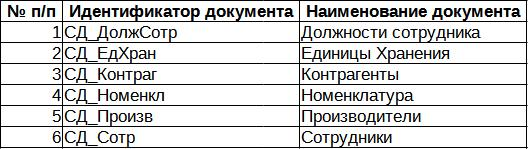
\includegraphics[]
            {_docs/СД.jpg}
        \caption{Каталог справочных документов}
        \label{fig:cd}
    \end{figure}

    Справочник <<Должности сотрудника>> - содержит должности сотрудника.
    Документ представлен в виде словаря данных (рисунок~\ref{fig:cd_DoljnCotr_tipi})
    и макета (рисунок~\ref{fig:cd_DoljnCotr_maket}).

    \begin{figure}[!h]
        \centering
        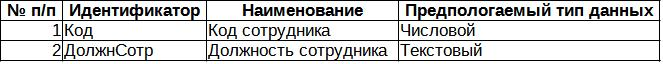
\includegraphics[]
            {_docs/СД_ДолжнСотр_типы.jpg}
        \caption{Словарь данных справочника <<Должности сотрудника>>}
        \label{fig:cd_DoljnCotr_tipi}
    \end{figure}

    \begin{figure}[!h]
        \centering
        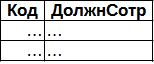
\includegraphics[]
            {_docs/СД_ДолжнСотр_макет.jpg}
        \caption{Макет справочника <<Должности сотрудника>>}
        \label{fig:cd_DoljnCotr_maket}
    \end{figure}

    \newpage

    Справочник <<Единицы хранения>> - содержит единицы хранения материала.
    Документ представлен в виде словаря данных (рисунок~\ref{fig:cd_EdXran_tipi})
    и макета (рисунок~\ref{fig:cd_EdXran_maket}).

    \begin{figure}[!h]
        \centering
        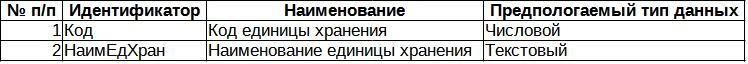
\includegraphics[]
            {_docs/СД_ЕдХран_типы.jpg}
        \caption{Словарь данных справочника <<Единицы хранения>>}
        \label{fig:cd_EdXran_tipi}
    \end{figure}

    \begin{figure}[!h]
        \centering
        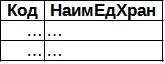
\includegraphics[]
            {_docs/СД_ЕдХран_макет.jpg}
        \caption{Макет справочника <<Единицы хранения>>}
        \label{fig:cd_EdXran_maket}
    \end{figure}

    Справочник <<Контрагенты>> - содержит информацию о контрагентах.
    Документ представлен в виде словаря данных (рисунок~\ref{fig:cd_Kontrag_tipi})
    и макета (рисунок~\ref{fig:cd_Kontrag_maket}).

    \begin{figure}[!h]
        \centering
        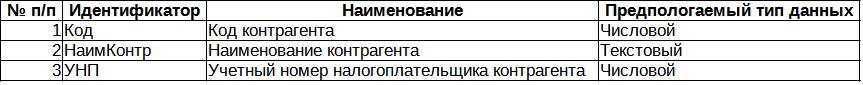
\includegraphics[width=16cm]
            {_docs/СД_Контраг_типы.jpg}
        \caption{Словарь данных справочника <<Контрагенты>>}
        \label{fig:cd_Kontrag_tipi}
    \end{figure}

    \begin{figure}[!h]
        \centering
        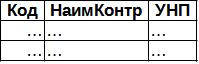
\includegraphics[]
            {_docs/СД_Контраг_макет.jpg}
        \caption{Макет справочника <<Контрагенты>>}
        \label{fig:cd_Kontrag_maket}
    \end{figure}

    Справочник <<Номенклатура>> - содержит информацию о материалах.
    Документ представлен в виде словаря данных (рисунок~\ref{fig:cd_Nomenkl_tipi})
    и макета (рисунок~\ref{fig:cd_Nomenkl_maket}).

    \begin{figure}[!h]
        \centering
        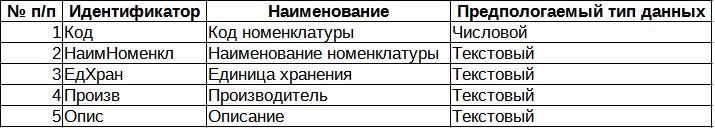
\includegraphics[width=16cm]
            {_docs/СД_Номенкл_типы.jpg}
        \caption{Словарь данных справочника <<Номеклатура>>}
        \label{fig:cd_Nomenkl_tipi}
    \end{figure}

    \begin{figure}[!h]
        \centering
        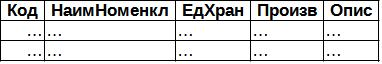
\includegraphics[]
            {_docs/СД_Номенкл_макет.jpg}
        \caption{Макет справочника <<Номеклатура>>}
        \label{fig:cd_Nomenkl_maket}
    \end{figure}

    \newpage

    Справочник <<Производители>> - содержит информацию о производителях.
    Документ представлен в виде словаря данных (рисунок~\ref{fig:cd_Proizv_tipi})
    и макета (рисунок~\ref{fig:cd_Proizv_maket}).

    \begin{figure}[!h]
        \centering
        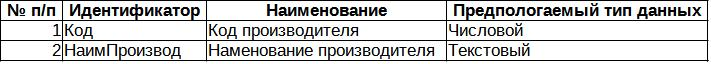
\includegraphics[width=16cm]
            {_docs/СД_Произв_типы.jpg}
        \caption{Словарь данных справочника <<Производители>>}
        \label{fig:cd_Proizv_tipi}
    \end{figure}

    \begin{figure}[!h]
        \centering
        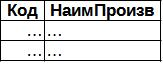
\includegraphics[]
            {_docs/СД_Произв_макет.jpg}
        \caption{Макет справочника <<Производители>>}
        \label{fig:cd_Proizv_maket}
    \end{figure}

    Справочник <<Сотрудники>> - содержит информацию о сотрудниках.
    Документ представлен в виде словаря данных (рисунок~\ref{fig:cd_Sotr_tipi})
    и макета (рисунок~\ref{fig:cd_Sotr_maket}).

    \begin{figure}[!h]
        \centering
        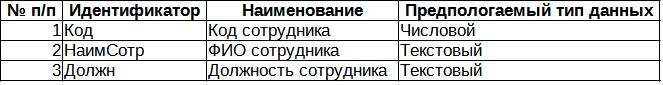
\includegraphics[]
            {_docs/СД_Сотр_типы.jpg}
        \caption{Словарь данных справочника <<Сотрудники>>}
        \label{fig:cd_Sotr_tipi}
    \end{figure}

    \begin{figure}[!h]
        \centering
        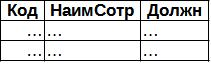
\includegraphics[]
            {_docs/СД_Сотр_макет.jpg}
        \caption{Макет справочника <<Сотрудники>>}
        \label{fig:cd_Sotr_maket}
    \end{figure}

    \subsubsection{Оперативные документы}

    Оперативные документы представлены в <<Каталоге оперативных документов>> (рисунок~\ref{fig:od}).
    
    \begin{figure}[!h]
        \centering
        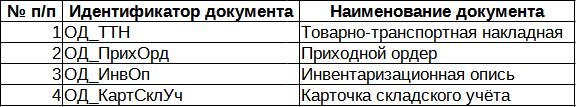
\includegraphics[]
            {_docs/ОД.jpg}
        \caption{Каталог оперативных документов}
        \label{fig:od}
    \end{figure}

    \newpage

    Оперативный документ <<Товарно-транспортная накладная>> - предназначена для учёта
    товарно-материальных ценностей (ТМЦ) при их перемещении с участием транспортных средств
    и является основанием для списания ТМЦ у грузоотправителя и оприходования их у грузополучателя.
    Документ представлен в виде словаря данных (рисунок~\ref{fig:od_TTH_tipi})
    и макета (рисунок~\ref{fig:od_TTH_maket}).

    \begin{figure}[p!h]
        \centering
        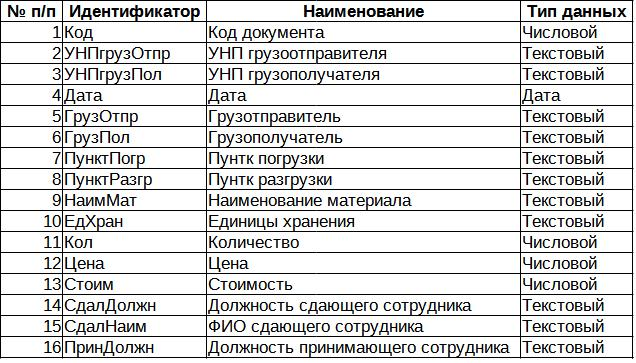
\includegraphics[]
            {_docs/ОД_ТТН_типы.jpg}
        \caption{Словарь данных документа <<Товарно-транспортная накладная>>}
        \label{fig:od_TTH_tipi}
    \end{figure}

    \begin{figure}[p!h]
        \centering
        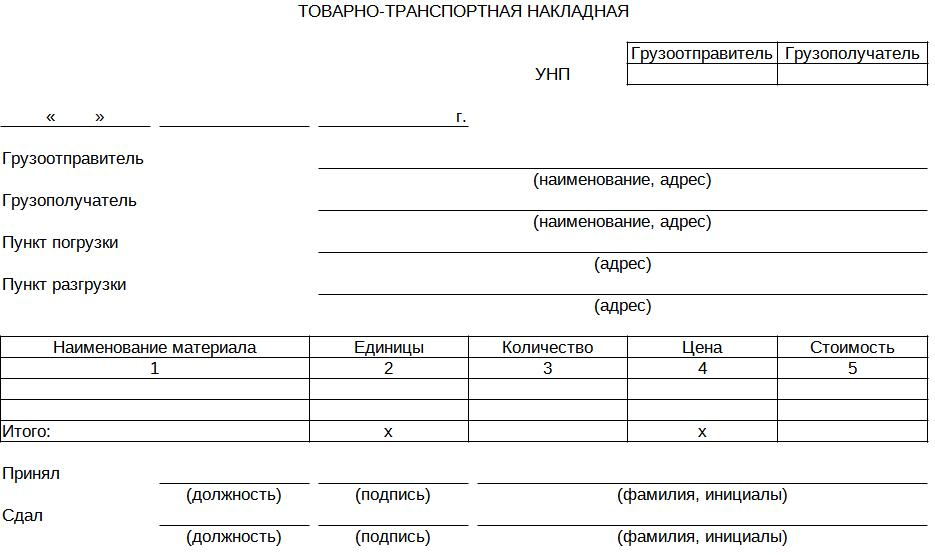
\includegraphics[width=16cm]
            {_docs/ОД_ТТН_макет.jpg}
        \caption{Макет документа <<Товарно-транспортная накладная>>}
        \label{fig:od_TTH_maket}
    \end{figure}

    \newpage

    Оперативный документ <<Приходный ордер>> - данным документов оформляется
    поступление наличных денежных средств в кассу предприятия.
    Документ представлен в виде словаря данных (рисунок~\ref{fig:od_PrihOrd_tipi})
    и макета (рисунок~\ref{fig:od_PrihOrd_maket}).

    \begin{figure}[p!h]
        \centering
        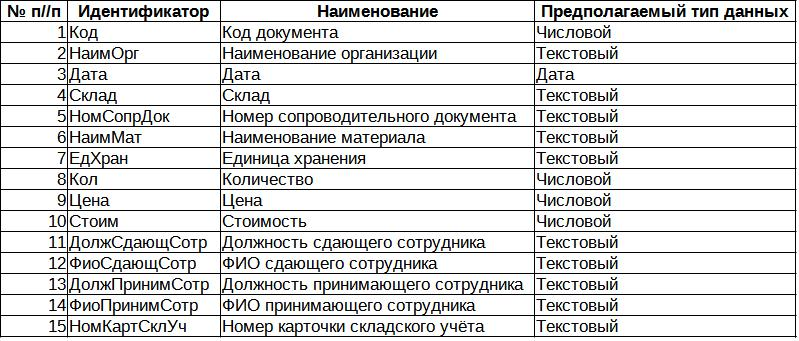
\includegraphics[]
            {_docs/ОД_ПрихОрд_типы.jpg}
        \caption{Словарь данных документа <<Приходный ордер>>}
        \label{fig:od_PrihOrd_tipi}
    \end{figure}

    \begin{figure}[p!h]
        \centering
        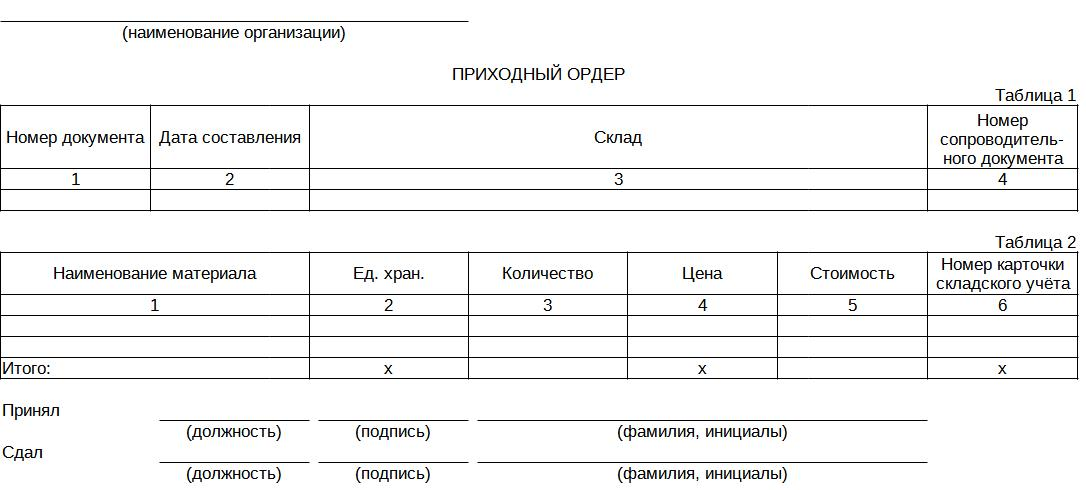
\includegraphics[width=16cm]
            {_docs/ОД_ПрихОрд_макет.jpg}
        \caption{Макет документа <<Приходный ордер>>}
        \label{fig:od_PrihOrd_maket}
    \end{figure}


    \newpage
    Оперативный документ <<Карточка складского учёта>> - применяется для учёта движения материалов на складе
    и заполняется материально отвественным лицом.
    Документ представлен в виде словаря данных (рисунок~\ref{fig:od_KartSklYch_tipi})
    и макета (рисунок~\ref{fig:od_KartSklYch_maket}).

    \begin{figure}[p!h]
        \centering
        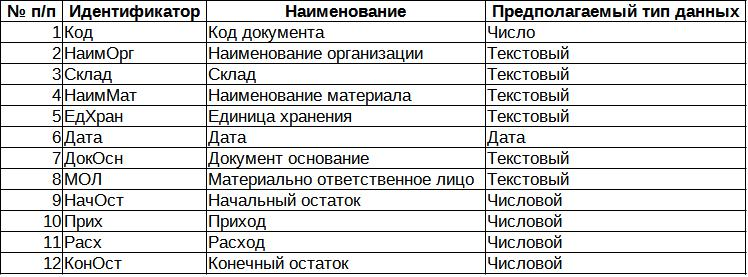
\includegraphics[]
            {_docs/ОД_КартСклУч_типы.jpg}
        \caption{Словарь данных документа <<Карточка складского учёта>>}
        \label{fig:od_KartSklYch_tipi}
    \end{figure}

    \begin{figure}[p!h]
        \centering
        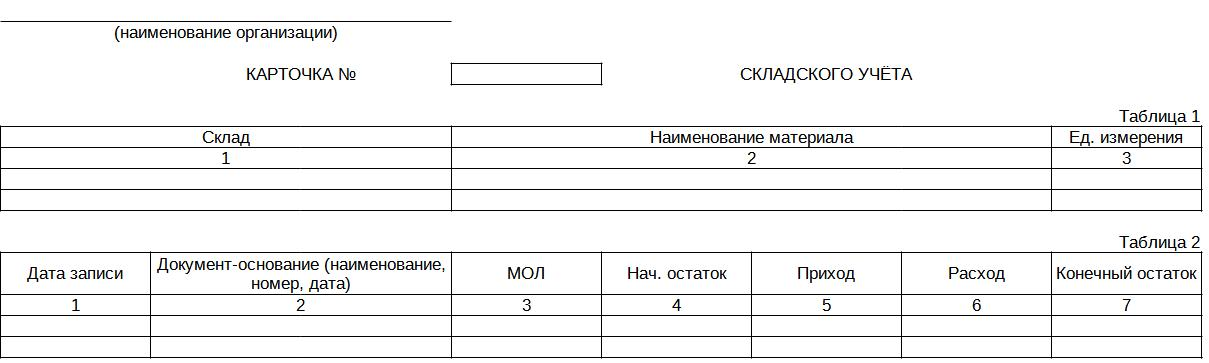
\includegraphics[width=16cm]
            {_docs/ОД_КартСклУч_макет.jpg}
        \caption{Макет документа <<Карточка складского учёта>>}
        \label{fig:od_KartSklYch_maket}
    \end{figure}

    \subsubsection{Отчётные документы}

    Отчётные документы представлены в <<Каталоге отчётных документов>> (рисунок~\ref{fig:OT}).
    
    \begin{figure}[!h]
        \centering
        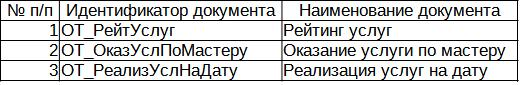
\includegraphics[]
            {_docs/ОТ.jpg}
        \caption{Каталог отчётных документов}
        \label{fig:OT}
    \end{figure}

    \newpage

    Отчётный документ <<Оборотно-сальдова ведомость товарно материальной ценности на дату>>
    - регистр бухгалтерского учёта, предназначен для контроля операций
    и сальдо по отчётам бухгалтерского учёта и составления бухгалтерской отчётности.
    Документ представлен в виде словаря данных (рисунок~\ref{fig:OT_OborSaldVed_tipi})
    и макета (рисунок~\ref{fig:OT_OborSaldVed_maket}).

    \begin{figure}[!h]
        \centering
        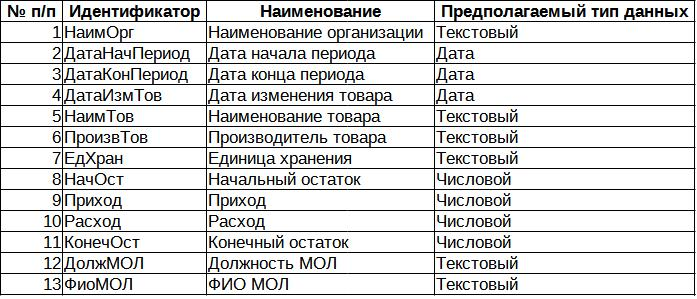
\includegraphics[]
            {_docs/ОТ_ОборСальдВед_типы.jpg}
        \caption{Словарь данных документа <<Оборотно-сальдова ведомость товарно материальной ценности на дату>>}
        \label{fig:OT_OborSaldVed_tipi}
    \end{figure}

    \begin{figure}[!h]
        \centering
        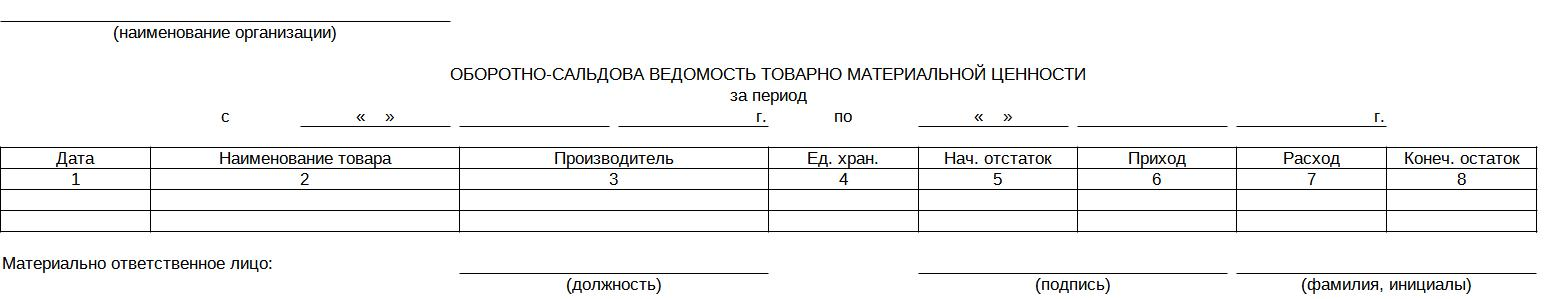
\includegraphics[width=16cm]
            {_docs/ОТ_ОборСальдВед_макет.jpg}
        \caption{Макет документа <<Оборотно-сальдова ведомость товарно материальной ценности на дату>>}
        \label{fig:OT_OborSaldVed_maket}
    \end{figure}

    \newpage

    Отчётный документ <<Рейтинг услуг>>
    - каждую неделю формируется и отражает отсортированные объемы реализации каждой услуги за указанные период.
    Документ представлен в виде словаря данных (рисунок~\ref{fig:OT_ReitYslyg_tipi})
    и макета (рисунок~\ref{fig:OT_ReitYslyg_maket}).

    \begin{figure}[!h]
        \centering
        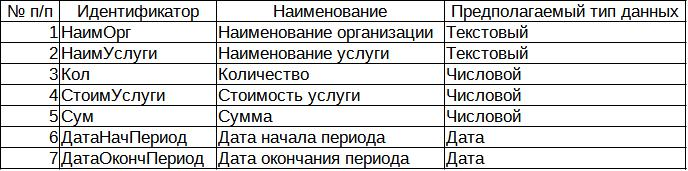
\includegraphics[]
            {_docs/ОТ_РейтУслуг_типы.jpg}
        \caption{Словарь данных документа <<Рейтинг услуг>>}
        \label{fig:OT_ReitYslyg_tipi}
    \end{figure}

    \begin{figure}[!h]
        \centering
        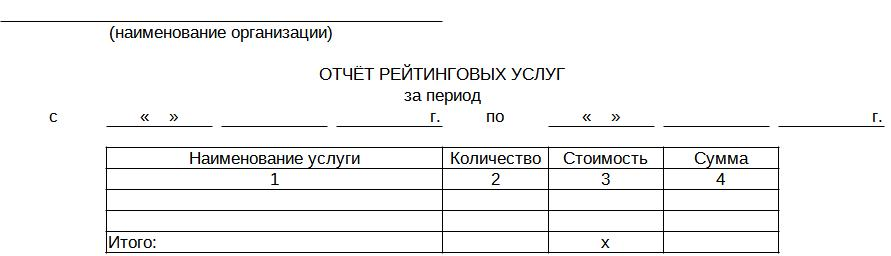
\includegraphics[width=16cm]
            {_docs/ОТ_РейтУслуг_макет.jpg}
        \caption{Макет документа <<Рейтинг услуг>>}
        \label{fig:OT_ReitYslyg_maket}
    \end{figure}

    \newpage

    Отчётный документ <<Оказание услуги по мастерам>>
    - каждую неделю формируется и отражает отсортированные объемы оказания услуг по каждому мастеру за указанные период.
    Документ представлен в виде словаря данных (рисунок~\ref{fig:OT_OkazYslPoMastery_tipi})
    и макета (рисунок~\ref{fig:OT_OkazYslPoMastery_maket}).

    \begin{figure}[!h]
        \centering
        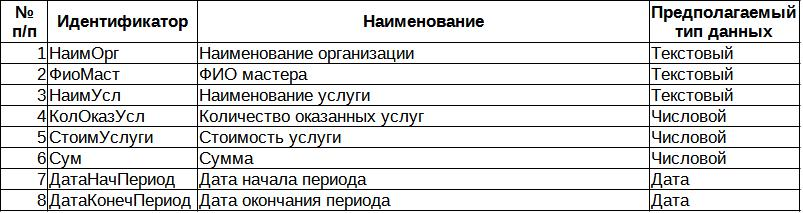
\includegraphics[]
            {_docs/ОТ_ОказУслПоМастеру_типы.jpg}
        \caption{Словарь данных документа <<Оказание услуги по мастерам>>}
        \label{fig:OT_OkazYslPoMastery_tipi}
    \end{figure}

    \begin{figure}[!h]
        \centering
        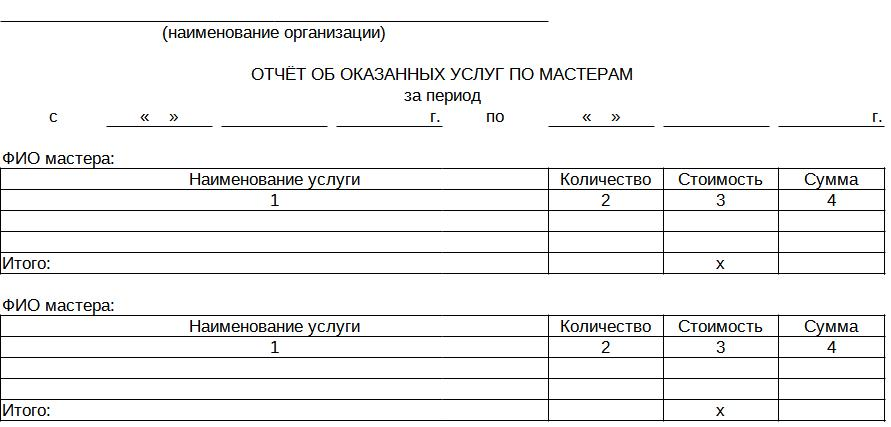
\includegraphics[width=14cm]
            {_docs/ОТ_ОказУслПоМастеру_макет.jpg}
        \caption{Макет документа <<Оказание услуги по мастерам>>}
        \label{fig:OT_OkazYslPoMastery_maket}
    \end{figure}

    \newpage

    Отчётный документ <<Реализация услуг на дату>>
    - документ, в котором хранится информация о всех оказанных услугах за определенный день.
    Документ представлен в виде словаря данных (рисунок~\ref{fig:OT_RealizYslNaDaty_tipi})
    и макета (рисунок~\ref{fig:OT_RealizYslNaDaty_maket}).

    \begin{figure}[!h]
        \centering
        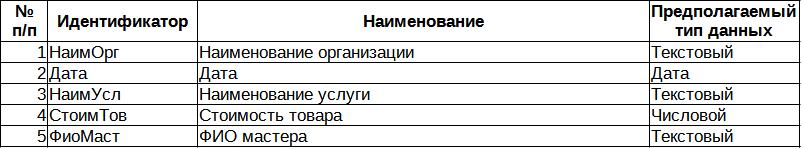
\includegraphics[]
            {_docs/ОТ_РеализУслНаДату_типы.jpg}
        \caption{Словарь данных документа <<Реализация услуг на дату>>}
        \label{fig:OT_RealizYslNaDaty_tipi}
    \end{figure}

    \begin{figure}[!h]
        \centering
        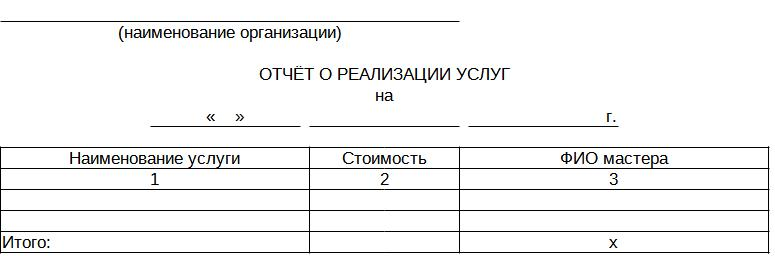
\includegraphics[]
            {_docs/ОТ_РеализУслНаДату_макет.jpg}
        \caption{Макет документа <<Реализация услуг на дату>>}
        \label{fig:OT_RealizYslNaDaty_maket}
    \end{figure}

    \newpage
    
    \subsection{Модель бизнес-процесса объекта автоматизации}
    \newpage

    %
    \section{РАЗРАБОТКА БАЗЫ ДАННЫХ}
    \subsection{Концептуальная модель}
    \subsection{Логическая модель}
    \subsection{Физическая модель}
    \newpage

    %
    \newpage
    \addcontentsline{toc}{section}{ЗАКЛЮЧЕНИЕ}
    \section*{ЗАКЛЮЧЕНИЕ}
    \newpage

    %
    \newpage
    \addcontentsline{toc}{section}{СПИСОК ИСПОЛЬЗОВАННЫХ ИСТОЧНИКОВ}
    \section*{СПИСОК ИСПОЛЬЗОВАННЫХ ИСТОЧНИКОВ}
    \begin{enumerate}    
        \item[1.] ARIS — Википедия
        - [Электронный ресурс]
        Режим доступа: \url{https://ru.wikipedia.org/wiki/ARIS}
        Дата~доступа:~07.03.2022.
        \item[2.] Информационная модель — Википедия
        - [Электронный ресурс]
        Режим доступа: \url{https://ru.wikipedia.org/wiki/%D0%98%D0%BD%D1%84%D0%BE%D1%80%D0%BC%D0%B0%D1%86%D0%B8%D0%BE%D0%BD%D0%BD%D0%B0%D1%8F_%D0%BC%D0%BE%D0%B4%D0%B5%D0%BB%D1%8C}
        Дата~доступа:~07.03.2022.
        \item[3.] Товарно-транспортная накладная — Википедия
        - [Электронный ресурс]
        Режим доступа: \url{https://ru.wikipedia.org/wiki/%D0%A2%D0%BE%D0%B2%D0%B0%D1%80%D0%BD%D0%BE-%D1%82%D1%80%D0%B0%D0%BD%D1%81%D0%BF%D0%BE%D1%80%D1%82%D0%BD%D0%B0%D1%8F_%D0%BD%D0%B0%D0%BA%D0%BB%D0%B0%D0%B4%D0%BD%D0%B0%D1%8F}
        Дата~доступа:~07.03.2022.
        \item[4.] Приходный кассовый ордер — Википедия
        - [Электронный ресурс]
        Режим доступа: \url{https://ru.wikipedia.org/wiki/%D0%9F%D1%80%D0%B8%D1%85%D0%BE%D0%B4%D0%BD%D1%8B%D0%B9_%D0%BA%D0%B0%D1%81%D1%81%D0%BE%D0%B2%D1%8B%D0%B9_%D0%BE%D1%80%D0%B4%D0%B5%D1%80}
        Дата~доступа:~07.03.2022.
        \item[5.] Карточка складского учета материальных ценностей М-17А 
        - [Электронный ресурс]
        Режим доступа: \url{https://blanki.by/catalog/zhurnaly/sklad/kartochka-skladskogo-ucheta-m-17a/}
        Дата~доступа:~07.03.2022.
        \item[6.] Оборотно-сальдовая ведомость — Википедия
        - [Электронный ресурс]
        Режим доступа: \url{https://ru.wikipedia.org/wiki/%D0%9E%D0%B1%D0%BE%D1%80%D0%BE%D1%82%D0%BD%D0%BE-%D1%81%D0%B0%D0%BB%D1%8C%D0%B4%D0%BE%D0%B2%D0%B0%D1%8F_%D0%B2%D0%B5%D0%B4%D0%BE%D0%BC%D0%BE%D1%81%D1%82%D1%8C}
        Дата~доступа:~07.03.2022.
    \end{enumerate}
    \newpage

    %
    \newpage
    \addcontentsline{toc}{section}{СПИСОК СОКРАЩЕНИЙ}
    \section*{СПИСОК СОКРАЩЕНИЙ}
    
    \begin{tabular}{ll} 
        ARIS    & architecture of integrated information system.\\
        ИС      & информационная система.\\
        МОЛ     & материально отвественное лицо.\\
        ОА      & объект автоматизации.\\
        ОП      & оперативный документ.\\
        ОТ      & отчётный документ.\\
        СП      & справочный документ.\\
        СУБД    & система управления базами данных.\\
        ТМЦ     & товарно-материальные ценности.\\
        БД      & база данных.\\
    \end{tabular}
    
    \newpage
\end{document}
